\documentclass{article}
%\documentclass{scrartcl}
\usepackage[czech]{babel}
\usepackage[utf8]{inputenc}
\usepackage{titling}
\newcommand{\subtitle}[1]{%
  \posttitle{%
    \par\end{center}
    \begin{center}\large#1\end{center}
    \vskip0.5em}%
}
\usepackage{graphicx}
\author{Jiří Kalvoda}
\date{}
\title{Propast Macocha}
\subtitle{Popis -- unikátní zeměpisný útvar}
\begin{document}
\maketitle
Propast Macocha je jednou z dominant Moravského krasu.
Nachází se samém centru této chráněné oblasti poblíž města Blanska.
I přesto, že se nejedná o nejhlubší propast v České republice, je Macocha tou nejnavštěvovanější.
Nejhlubší je Hranická propast se svojí hloubkou minimálně 470 metrů.
Její dno je však zatopené.

%První sestup do propasti uskutečnil již v roce 1723 mnichem Lazarem Schopperem.

Macocha pravděpodobně vznikla prolomením klenby jeskynního dómu.
Úlomky a suť z klenby je stále patrná na jejím dně v podobě menších i větších kamenů nepravidelného neopracovaného tvaru.
I když na dno slunce svítí pouze v omezeném množství, roste tu specifický zelený porost.
Propast je 137 metrů hluboká 170 metrů dlouhá a 70 široká.
Na jejím dně se nachází dvě krasová jezírka charakteristická svojí azurově-zelenou barvou.
Menší z jezírek, nazvané Horní, se nachází těsně u severní stěny. Při nízkém stavu vody se v jeho středu vynořuje velký kus skály. Odsud voda pokračuje kaskádovitým potůčkem do Dolního jezírka, které dosahuje hloubky okolo padesáti metrů.
Do jezírek přivádí vodu systém systém ponorných říček Amatérské jeskyně.
Z propasti voda odtéká jako řeka Punkva zahloubená v Punkevní jeskyni.
Její tok je ovšem uměle narušen z důvodu umožnění plavby po její hladině v jeskyni.
Stěny propasti jsou tvořeny vápencovými skalními stěnami, které částečně zarůstají mechy a lišejníky.
Severní stěna postupně ve své horní části přechází v lesní porost, zatímco jih propasti strmě stoupá až na okolní úroveň.
Na této straně byl vybudován vyhlídkový můstek, který svojí hranou zasahuje až nad samotnou propast.
Turisté mohou stát na jeho dřevěné podlaze položené na kovových nosnících.
O bezpečnost se stará ozdobně litinové zábradlí.
Výhled do propasti je také umožněn z dolního můstku, pro jehož návštěvu je nutné sestoupit svah ze západní strany.
Tímto místem byl do propasti proveden první sestup, protože terén z této strany je nejméně sklopený a vertikální skalnatý úsek je vysoký jen pár desítek metrů.
Tento můstek je převážně betonový obložen kameny a ozdoben zábradlím ve stejném stylu.
Dno propasti se dá navštívit při prohlídce navazujících punkevních jeskyň.


Název propasti vznikl zkomolením slova macecha. Dle pověsti měla macecha shodit do propasti svého nevlastního syna.
Ten se však zachytil pod hranou. Poté, co o událostech řekl vesničanům, kteří ho zachránili, svrhli macechu do propasti.
\section{Zdroje}
\emph{Macocha} [online], poslední aktualizace 12. prosince 2019 [cit. 1. 1. 2020], Wikipedie. Dostupné z WWW: $\left<\right.$http://cs.wikipedia.org/wiki/Macocha$\left.\right>$

\ \\
\begin{center}
	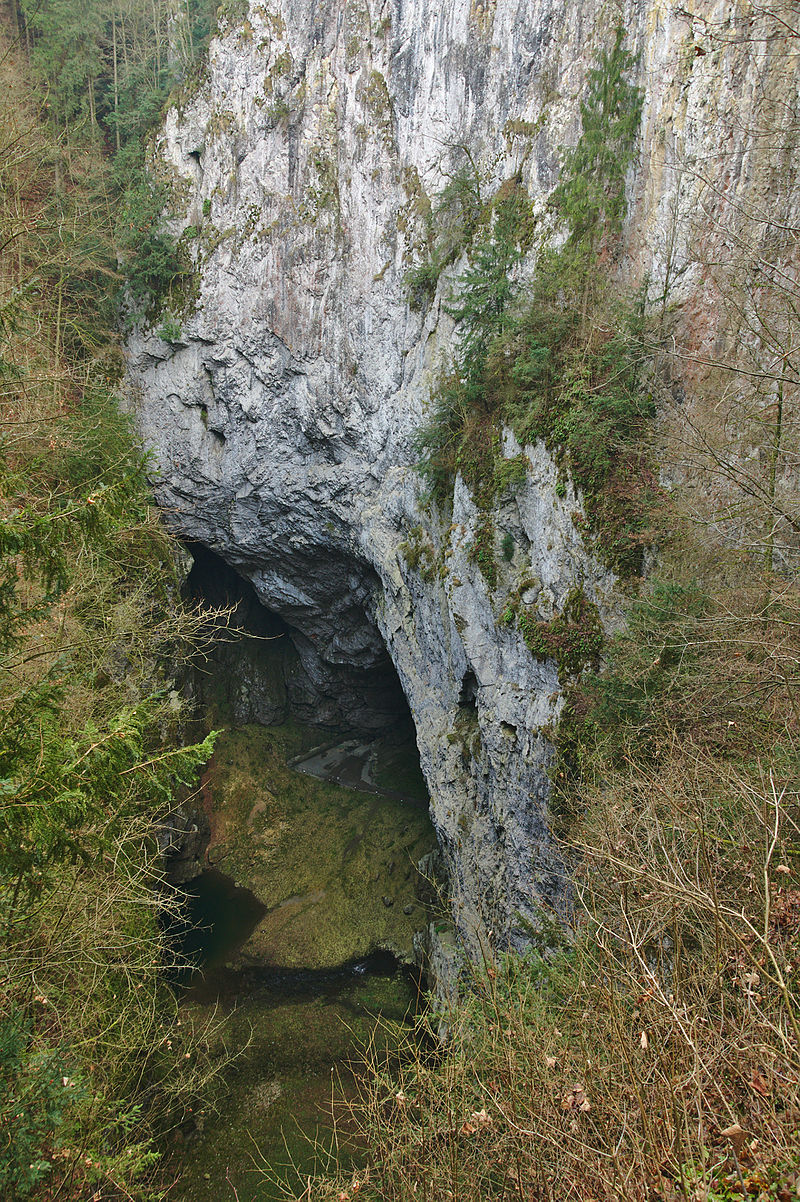
\includegraphics[scale=01]{macocha1.jpg}
	\ \\
	\ \\

	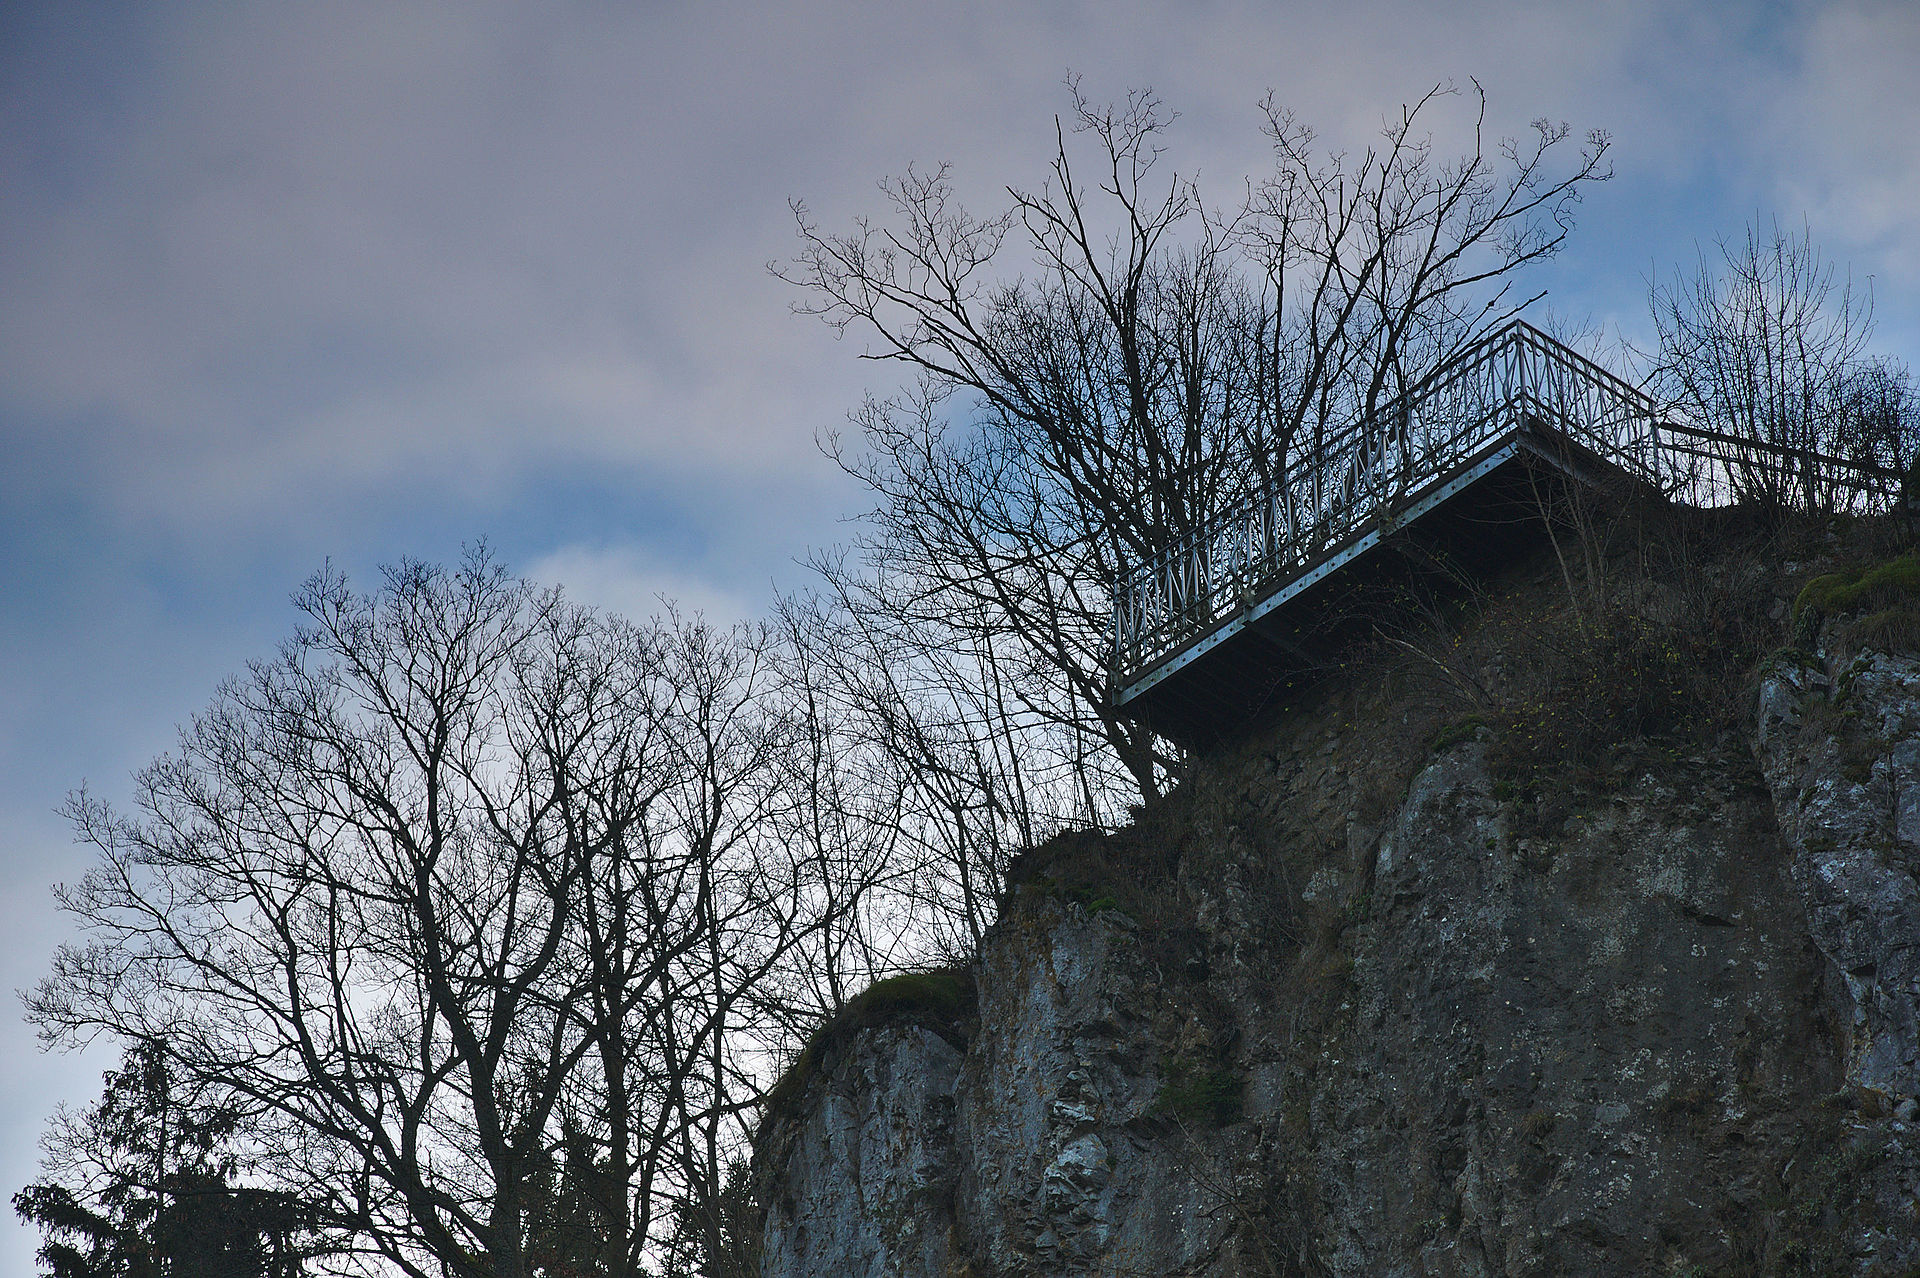
\includegraphics[scale=0.5]{macocha2.jpg}
\end{center}
\end{document}
